% This version of CVPR template is provided by Ming-Ming Cheng.
% Please leave an issue if you found a bug:
% https://github.com/MCG-NKU/CVPR_Template.

%\documentclass[review]{cvpr}
\documentclass[final]{cvpr}

\usepackage{times}
\usepackage{epsfig}
\usepackage{graphicx}
\usepackage{amsmath}
\usepackage{amssymb}

% Include other packages here, before hyperref.
%% 代码和图片的包
\usepackage{listings}
\usepackage{xcolor}
\usepackage{graphicx}
\usepackage{float}
\lstset{
    numberstyle= \tiny, 
    keywordstyle= \color{red!100!green!90!blue!70},
    commentstyle= \color{red!50!green!50!blue!50}, 
    stringstyle= \color{red!20!green!80!blue!80},
    frame=shadowbox, % 阴影效果
    rulesepcolor= \color{ red!20!green!20!blue!20} ,
    escapeinside=``, % 英文分号中可写入中文
    xleftmargin=2em,xrightmargin=0em, aboveskip=1em,
    framexleftmargin=2em,
    language=matlab
} 
%% 伪代码的包
\usepackage{algorithm}  
\usepackage{algpseudocode}  
\usepackage{amsmath}  
\renewcommand{\algorithmicrequire}{\textbf{Input:}}
\renewcommand{\algorithmicensure}{\textbf{Output:}} 

% If you comment hyperref and then uncomment it, you should delete
% egpaper.aux before re-running latex.  (Or just hit 'q' on the first latex
% run, let it finish, and you should be clear).
\usepackage[pagebackref=true,breaklinks=true,colorlinks,bookmarks=false]{hyperref}


\def\cvprPaperID{****} % *** Enter the CVPR Paper ID here
\def\confYear{CVPR 2021}
%\setcounter{page}{4321} % For final version only


\begin{document}

%%%%%%%%% TITLE
\title{Lecture Note for Seam Carving}

\author{ender507\\
Sun Yat-sen University (SYSU)\\
China\\
{\tt\small hutx@mail2.sysu.edu.cn}
}

\maketitle


%%%%%%%%% ABSTRACT
\begin{abstract}
   Seam Carving \cite{ref4} is a technique which allow us to resize pictures in order to display these pictures in devices which have different screen size or display resolution ratio. Compared to previous approaches of picture resizing, which may change the shape of the object in the picture, or cut up some of the important parts in the picture, Seam Carving can remain the important parts as it used to be. By simply calculate the importance of every single pixels, Seam Carving just delete the path of pixels which share the least important so that the picture can stay what it looks like at the beginning as possible while resizing.
\end{abstract}

%%%%%%%%% BODY TEXT
\section{Background and related works}

 In our daily life, we have numerous kinds of devices which have different screen size or display resolution ratio. If we want to display a picture with different devices, we must change the size of the picture in order to make it fit for the device. However, the result of normal ways of picture resizing is always unsatisfying. 
 
 One of the widely used approach is scale, which can be realise by many algorithms such as linear interpolation \cite{ref1} , nearest neighbor scaling \cite{ref2} , and spline interpolation \cite{ref3} .All these algorithms have one common disadvantage, that is, the object in the picture will change its shape. If the input picture and the output picture have different ratio of aspect ratio, those objects will be compressed or stretched, which makes their appearance is not what they used to be. We always want to keep the object which keeps the most information of the picture stay what it looks like as in the input picture.

Another method is to crop the picture, so that those less important part can be cut off and important object can be retained and keeps the same appearance. Despite it, it is hard for devices to distinguish the important part, and crop pictures automatically. Besides, just think of a picture, which has a important object in the left side and another is in the right of the picture. If the picture is required to reduce its width, the only way is to crop the middle of the picture, and that will make the picture raise a gap in the middle.

Above all, a content-aware resizing operator is required. Should not only the picture can be resized, but also the important content can be kept. In another word, the resized picture can represent the previous picture as good as possible. New picture is supposed to adhere to the geometric constraints and preserve the important content and structures in the picture. Here we have a technique named Seam Carving, which is able to solve our problems.

%-------------------------------------------------------------------------
\section{Introduction to Seam Carving}
In this section, I am going to talk about the basic ideas of Seam Carving and how it works in details. In order to describe it particularly and concise, I will take the problem of reduce the width of the input picture as an example. Following parts are corresponding to every single steps of Seam Carving.
\subsection{Definition of importance}
If we want to keep the important parts of the picture, the first question is how to decide which part is important and which is not. Is it a salient object in the picture, or it is the part that our eyes will fixate once we look at the picture? No matter what it is, we must define it in a digital way. That means our computer can justify which part is less important and delete it.

Here we have a function called energy function. By giving input picture, the function is able to calculate the importance of every single pixels of the picture. So this function is how we define the importance of the picture. But how to design a good function to present the importance correctly? Nowadays, we got good machine learning algorithms and computers which have strong power. We can give the input pictures and corresponding importance picture labels, training a model by SVM or deep neural network to achieve the function. Or, we can simply use the gradient of the picture to define its importance.

Gradient-based definition of importance has many advantages. Apparently, it can preserve strong contours, which is in line with our intuition of what a important object is. In fact, human vision is so sensitive to edges that we always ignore smooth areas. At the same time, gradient is easy to calculate, which can simplify the method and accelerate the speed of the whole algorithm. 

Here is the definition of importance, or we can call it energy function:
$$
E(I)=|\frac{\partial}{\partial x}I|+|\frac{\partial}{\partial y}I|
$$

That is the sum of the absolute values of the gradient in the x-axis and the y-axis of a pixel. If the pixel has three or more color channels, just calculate the energy function in every channel and sum them all or solve the average value to present the total importance of the pixel. Let us take RGB channel as an example:
$$
E(I)=|\frac{\partial I_R}{\partial x}|+|\frac{\partial I_R}{\partial y}|+|\frac{\partial I_G}{\partial x}|+|\frac{\partial I_G}{\partial y}|+|\frac{\partial I_B}{\partial x}|+|\frac{\partial I_B}{\partial y}|
$$

After processing the input picture by energy function, now we have all the importance values of every pixels, which make up a energy picture.  

%------------
\subsection{Remove the less important part}
Since we have got all of the importance values of the input picture, now we need to decide which part to be deleted. Of course we are going to remove the part that has less importance, but how big it should be? If every time we just simply delete a pixel which is the least important one in the picture, the left pixels can not make a whole picture. Then how about delete every least important pixels in each row? That can be achieved easily, but as a result, the left part's shape will change. 

If we want to reduce the width of the input picture, for sure each time we are supposed to delete a pixel in each row, but we also need to pick up proper pixels  so that after deleting, the left picture has no gaps or intervals. That can be achieved if removed pixels in adjacent rows are also adjacent. That means if we remove one pixel whose coordinate is $(i,j)$ which $i$ and $j$ is the id of row and column, in the next row, the pixel to be removed has to have the coordinate of $(i+1, j-1)$, $(i+1, j)$, or $(j+1, j+1)$. That is what we call {\bf adjacent pixels}.

On account of removing those adjacent pixels, every time we will remove a curve from the input picture (Sometimes the curve can also be a straight line). So we should pay attention to the importance of a whole curve instead of a single pixel. The curve has least importance is to be deleted. Every time, we remove a curve from the input picture, and use the new picture as input picture, calculate its energy function and the least important curve again, we can remove another curve. By doing these iteratively, we can reduce the size of previous picture continuously.

\subsection{Find the curve by dynamic programming}
As we mentioned above, we need to calculate the importance of every curve in the picture in order to remove the least important one. However, it is very inefficient to compute those values directly. In fact, for a picture whose size is $m\times n$, it takes the time complexity of $n\times 3^m$ to calculate all paths' energy. Thankfully, this issue can be handled easily by using the technique of dynamic programming and finally, its time complexity can be reduced to only $m\times n$.

We can simply use a matrix $EC$, in which the value of $EC_{i,j}$ means how many energy is cumulated from the top of the picture to the pixel positioned in $(i,j)$. And we use another matrix $PM$ to present the path that has least energy. In $PM$, the value of $PM_{i,j}$ means to approach least energy, the pixel $(i-1, PM_{i,j})$ must go to the pixel $(i,j)$ in the path.

Since for each pixel in the picture's first row has cumulated energy which is as same as the energy itself kept, we can initialize the matrix $EC$'s first row as the energy map $E$'s first row, and $PM$'s first row is all initialized to -1 which means the end of path. Then we just traverse all pixels of the picture from top to bottom and from left to right and update all matrix mentioned above by keeping following rules.Set 
$$ec = \min({EC(i-1,j-1),EC(i-1.j),EC(i-1,j+1)})$$
then we got:
$$
EC_{i,j}=E_{i,j}+ec
$$
$$
PM_{i,j}=
\left\{\begin{matrix}{}
j-1,\quad if \quad EC(i-1,j-1)=ec\\
j,\quad if \quad EC(i-1,j)=ec\\
j+1,\quad if \quad EC(i-1,j+1)=ec\\
\end{matrix}\right.
$$

Here is the pseudocode:
\begin{algorithm}[htb]  
  \caption{Calculate $EC$ and $PM$}  
  \begin{algorithmic}[1]  
    \Require
    The energy map $E$;
    The size of raw picture $m\times n$;
    \Ensure  
    The cumulated energy map $EC$; 
    The path map $PM$;
    \State assign$i=1,j=1$;  
    \State calculate $ec$ as the minimal number in $EC(i-1,j-1)$, $EC(i-1.j)$ ,and $EC(i-1,j+1)$
    \State $EC_{i,j}=E_{i,j}+ec$ 
    \State if $EC(i-1,j-1)=ec$,$PM_{i,j}=j-1$;if $EC(i-1,j)=ec$,$PM_{i,j}=j$;if $EC(i-1,j+1)=ec$,$PM_{i,j}=j+1$ 
    \State if $i==m,j==n$, goto return; if $j==n$, then assign $i=i+1,j=1$, goto2; else assign $j=j+1$, goto2.\\
    \Return $EC$, $PM$;
  \end{algorithmic}  
\end{algorithm}

You can see a picture and its energy map and cumulated energy map in Figure \ref{pic0-1}, Figure \ref{pic0-2}, and Figure \ref{pic0-3}.

\begin{figure}
\begin{center}
    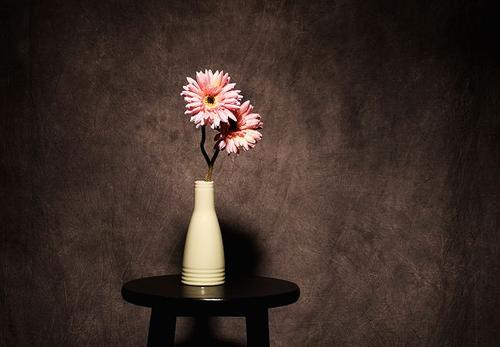
\includegraphics[scale=0.3]{pics/2-1.jpg}
    \caption{Picture1}
    \label{pic0-1}
    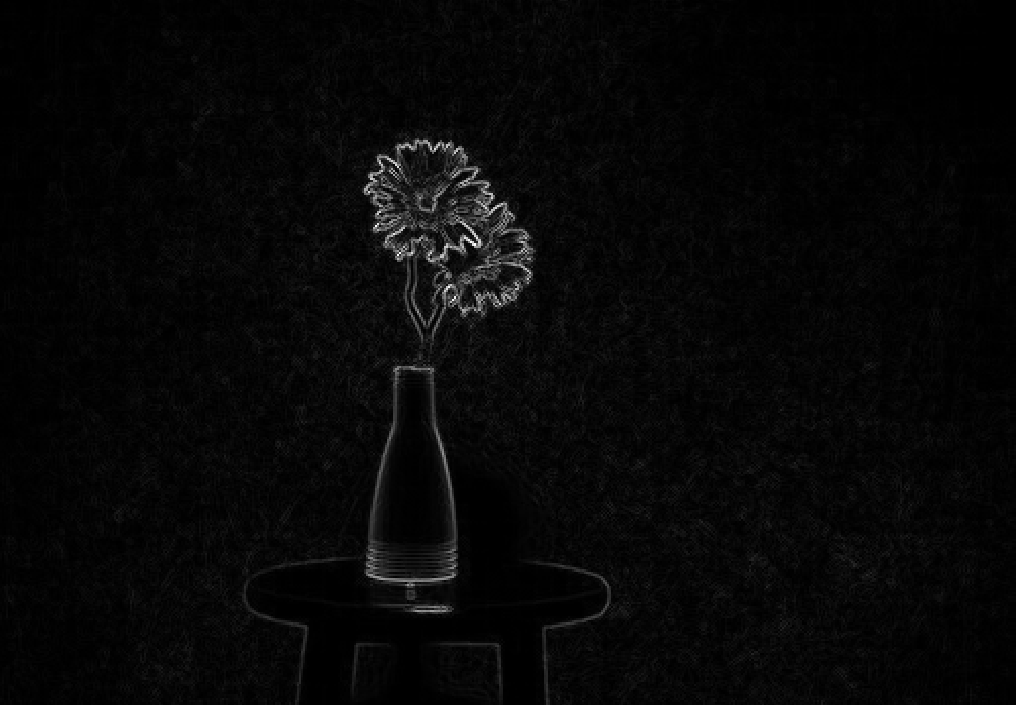
\includegraphics[scale=0.15]{pics/0-2.png}
    \caption{Picture1's energy map}
    \label{pic0-2}
    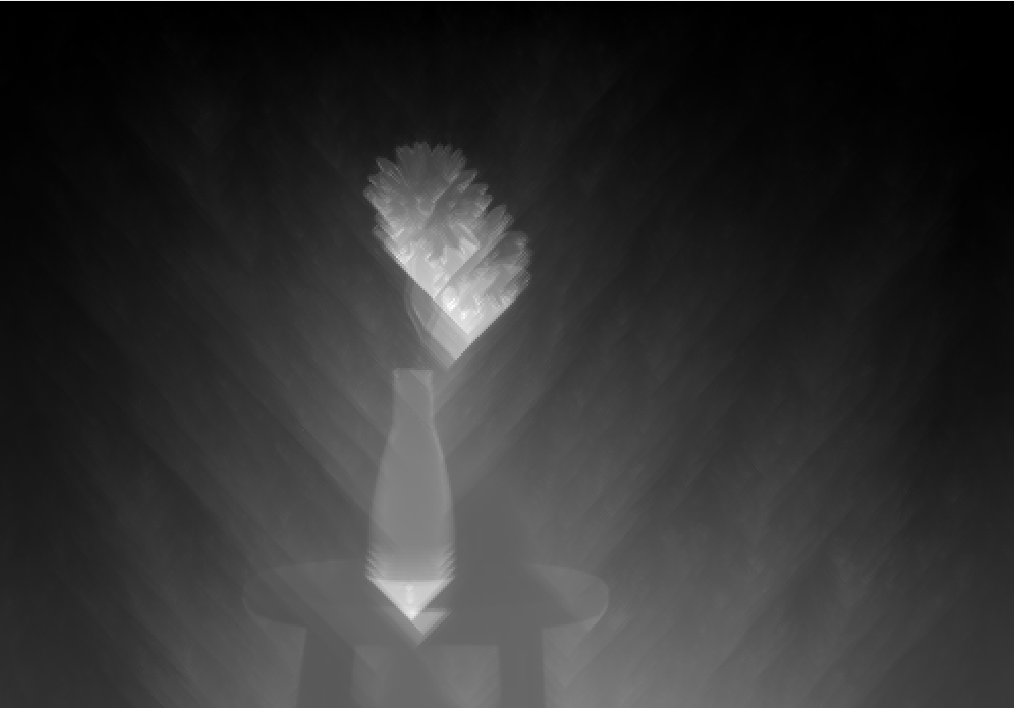
\includegraphics[scale=0.15]{pics/0-3.png}
    \caption{Picture1's cumulated energy map}
    \label{pic0-3}
\end{center}
\end{figure}

After we calculate all values in $EC$ and $PM$, we need to find the position of the values in $EC$'s last row which holds the minimal value in this row. The value presents the minimal energy among all paths is keeping. Let us assume its position is $(i_0,j_0)$, and by finding the value of $PM_{i,j}$, we can easily find another pixel's position in the path to be removed. That is $(i_1, j_1)$, where $i_1 = i_0 - 1$ and $j_1=PM(i_0,j_0)$. Similarly, we have another pixel $(i_2,j_2)$ to be removed where $i_2 = i_1 - 1$ and $j_2 = PM(i_1,j_1)$. By following the rules, finally we will get a group of pixels $(i_0,j_0)$...$(i_{m-1},j_{m-1})$, then we just delete them all.
\begin{algorithm}[htb]  
  \caption{Delete the path contains least energy}  
  \begin{algorithmic}[1]  
    \Require
    The cumulated energy map $EC$; 
    The path map $PM$;
    The raw picture $img$;  
    \Ensure  
    The result of deleting $img$'s path that contains least energy, as $img'$;
    \State assign $img' = img$
    \State assign $i$ is the serial number of $img$'s last row, and $j$ is the serial number of the position of the minimal value in $EC$'s last line;  
    \State delete the pixel $(i,j)$ from $img'$ 
    \State if $i==1$, goto return
    \State assign $i=i-1$, $j=PM(i,j)$, and goto 3;\\  
    \Return $img'$;  
  \end{algorithmic}  
\end{algorithm}

In effect, we removed one pixel from each row, and that means the size of the picture is reduced from $m\times n$ to $m\times(n-1)$. That is how Seam Carving works. Repeatedly, we take the new picture as an input picture, calculate its energy map, cumulate energy map, and path map again, we can find and delete another path which contains the least energy among all paths to make the picture get smaller until the picture's size if good enough. In preceding part of the text, I just introduced how to reduce the number of column of the picture, but the technique can applied be used to reduce the number of rows. We can reduce the size optionally as long as we want.

Here is the pseudocode of Seam Carving:
\begin{algorithm}[htb]  
  \caption{Seam Carving}  
  \begin{algorithmic}[1]  
    \Require
    The raw picture $img$; 
    The size of the raw picture $m\times n$;
    The size required $m'\times n'$;  
    \Ensure  
    The resized picture $img'$;  
    \State Calculate the gradient map of $img$ as $E$;  
    \State use matrix $EC$ to calculate the cumulate energy of each path from the top to the bottom or from the right side to the left side
    \State while calculate $EC$, use $PM$ to record the path that holds least energy;  
    \State delete the path from the picture $img$ to achieve $img'$;  
    \State if $img'$'s size is not as same as $m'\times n'$, assign $img = img'$ and goto 1\\  
    \Return $img'$;  
  \end{algorithmic}  
\end{algorithm}
%-----------------------------
\section{Code implementation}
Now I am going to show you how to implement Seam Carving by coding. I use the platform matlab and the version is 2020b, and I write all the codes by myself. You can obtain the full version of my codes and picture resources used in my codes in \url{https://github.com/ender507/My-Small-Program-Collection/tree/main/Seam%20Carving}.

\subsection{Picture loading and preprocessing}
At first, we load the picture and turns the pixel values from $[0,255]$ to $[0,1]$, then we get and save the previous size of the picture as `hei1', `wid1', and `dep2'. As an exmaple, we set `wid2' to be half of `wid1', which means the output picture's width is half of the previous picture. `wid\_now' presents the instant width of the picture being processing.
\begin{lstlisting}
% load the picture
img = im2double(imread("1.jpg"));
[hei1, wid1, dep1] = size(img);
% show the previous picture
imshow(img);    
figure;
% width to be reduced to half
wid2 = round(wid1/2);
wid_now = wid1;
\end{lstlisting}

In order to show how Seam Carving has a better performance compared to other common technique, here I used the technique of interpolation to reduce the width of the picture. If the column's serial number is odd, this column will be kept. Otherwise, the column will be removed if it got a even serial number. Here is the code to implement this:
\begin{lstlisting}
tmp_pic = img(:,1:2:wid1,:);
subplot(1,2,1)
imshow(tmp_pic);
\end{lstlisting}

Then we can start to process the picture with Seam Carving.
\subsection{Calculate the energy map}
Since at one time, Seam Carving just remove one path from the picture, but always we need to remove many paths from the picture, so following steps are in a loop:
\begin{lstlisting}
while wid_now ~= wid2
\end{lstlisting}
and in this loop, `wid\_now' reduce by 1 at each time. 

Now we are going to calculate the energy map. As mentioned before, for pictures holding 3 or more color channels, we can simply calculate the energy map of each channel and sum them all. As the codes go like this:
\begin{lstlisting}
[gx1, gy1] = gradient(img(:,:,1));
[gx2, gy2] = gradient(img(:,:,2));
[gx3, gy3] = gradient(img(:,:,3));
E = abs(gx1) + abs(gy1)...
    + abs(gx2) + abs(gy2)...
    + abs(gx3) + abs(gy3);
\end{lstlisting}

In `img(:,:,1)', `img(:,:,2)', and `img(:,:,3)', the thrid parameter divide the picture into red, green, blue channel respectively. The built-in function `gradient' will return the gradients in horizontal and vertical direction. Take the absolute values of these maps and sum them all, we can ultimately get the energy map $E$.

\subsection{Update EC and PM}
Let us initialize matrix $EC$ and $PM$ first.
\begin{lstlisting}
EC = zeros(hei1, wid_now);
PM = zeros(hei1,wid_now);
EC(1,:) = E(1,:);
\end{lstlisting}

In matlab, the first index value is 1 instead of 0, so we can use 0 to present the end of the path.
Now we can update every value in $EC$ and $PM$ using the approach of dynamic programming as we mentioned before. The order of traverse is like this:
\begin{lstlisting}
for i = 2:hei1
    for j = 2: wid_now-1
        ...
    end
end
\end{lstlisting}

In the inner loop, we have three cumulate energy values:
\begin{lstlisting}
tmp1 = EC(i-1, j-1);
tmp2 = EC(i-1, j);
tmp3 = EC(i-1, j+1);
\end{lstlisting}

And $EC$ and $PM$ are supposed to be updated by:
\begin{lstlisting}
if tmp1 < tmp2 && tmp1 < tmp3
    EC(i, j) = tmp1 + E(i, j);
    PM(i, j) = j-1;
elseif tmp2 < tmp1 && tmp2 < tmp3
    EC(i, j) = tmp2 + E(i, j);
    PM(i, j) = j;
else
    EC(i, j) = tmp3 + E(i, j);
    PM(i, j) = j+1;
end
\end{lstlisting}

Maybe you have found I start the loop at 2 and end it at `wid\_now-1', that is for the reason that in the first and the last column, we cannot calculate all values of `tmp1', `tmp2' and `tmp3', the indices will overstep the boundary otherwise.

The first column should be handled like this:
\begin{lstlisting}
tmp1 = EC(i-1, 1);
tmp2 = EC(i-1, 2);
if tmp1 < tmp2
    EC(i, 1) = tmp1 + E(i, 1);
    PM(i, 1) = 1;
else
    EC(i, 1) = tmp2 + E(i, 1);
    PM(i, 1) = 2;
end
\end{lstlisting}

And similarly, we deal with the last column as following:
\begin{lstlisting}
tmp1 = EC(i-1, wid_now-1);
tmp2 = EC(i-1, wid_now);
if tmp1 < tmp2
    EC(i, wid_now) = tmp1...
    + E(i, wid_now);
    PM(i, wid_now) = wid_now-1;
else
    EC(i, wid_now) = tmp2...
    + E(i, wid_now);
    PM(i, wid_now) = wid_now;
end
\end{lstlisting}

\subsection{Find and delete the path}
Now we have figured out all values in matrix $EC$ and $PM$, and we are supposed to find the path containing least cumulated energy and remove it from the picture. 
First we can easily find the position that holds the minimal value in $EC$'s last row. That means the path we need contains the pixel in this position. That's $(i_0,j_0)$ mentioned before. And we just need to find the next position in the path. By simply get the value of $PM_{I_0,j_0}$ we can get $j_1$, and $i_1 = i_0-1$. So we get the next pixel to be remove, that's $(i_1,j_1)$. By this way ,we can gradually delete the whole path.

\begin{lstlisting}
energy_min = min(EC(hei1, :));
min_pos=find(EC(hei1,:)==energy_min);
tmp_pic=zeros(hei1, wid_now-1, dep1);
for i = hei1:-1:2
    tmp = img(i,:,:);
    tmp_pic(i,:,:) = tmp(:,[1:...
    min_pos-1,min_pos+1:wid_now],:);
    min_pos = PM(i, min_pos);
end
tmp = img(1,:,:);
tmp_pic(1,:,:) = tmp(:,[1:...
min_pos-1,min_pos+1:wid_now],:);
img = tmp_pic;
\end{lstlisting}
At the end of the loop, we finally get the output picture, and display it for comparison.
\begin{lstlisting}
subplot(1,2,2);
imshow(img);
\end{lstlisting}

%------------
\section{Presentation of results}
In this section, I picked up some pictures in the Internet, and reduced their width to a half by respectively using the technique of interpolation and Seam Carving. I an going to show you the raw picture and the two processed pictures to show how Seam Carving have a better performance than other techniques.

For each picture, the order that I show is to be: the raw picture, the interpolation processed one, and the Seam Carving processed one.
\begin{figure}
\begin{center}
   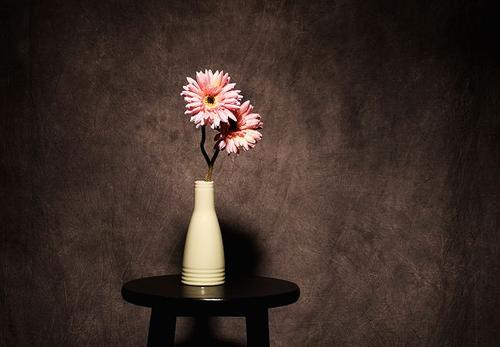
\includegraphics[scale=0.3]{pics/2-1.jpg}
    \caption{The raw picture1}
    \label{pic2-1}
    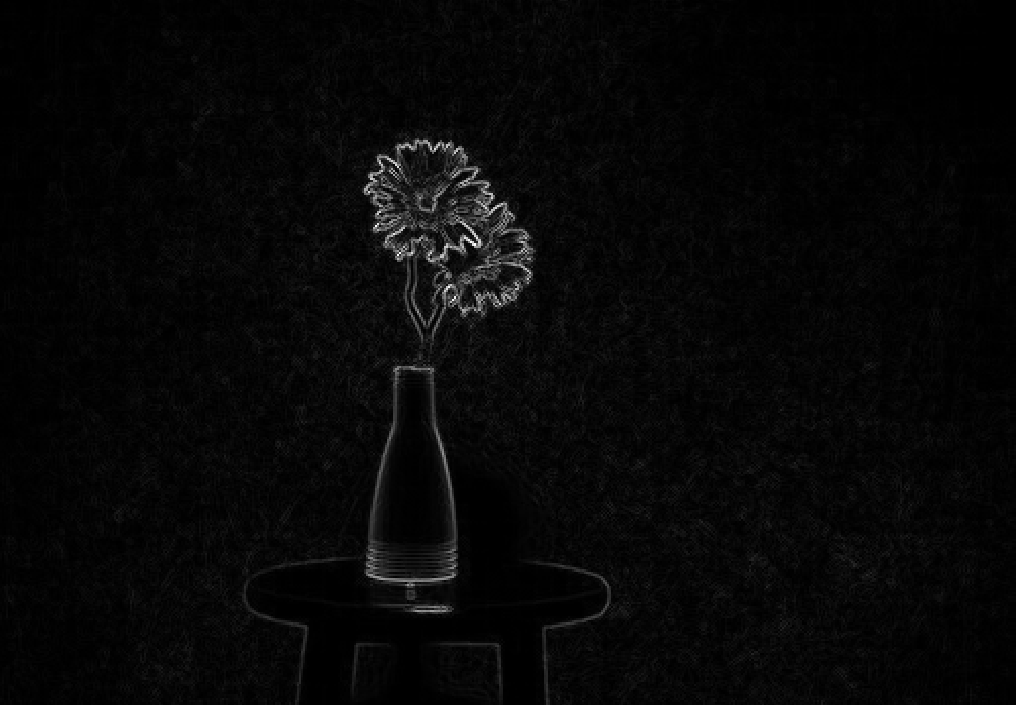
\includegraphics[scale=0.15]{pics/0-2.png}
    \caption{Picture1's energy map}
    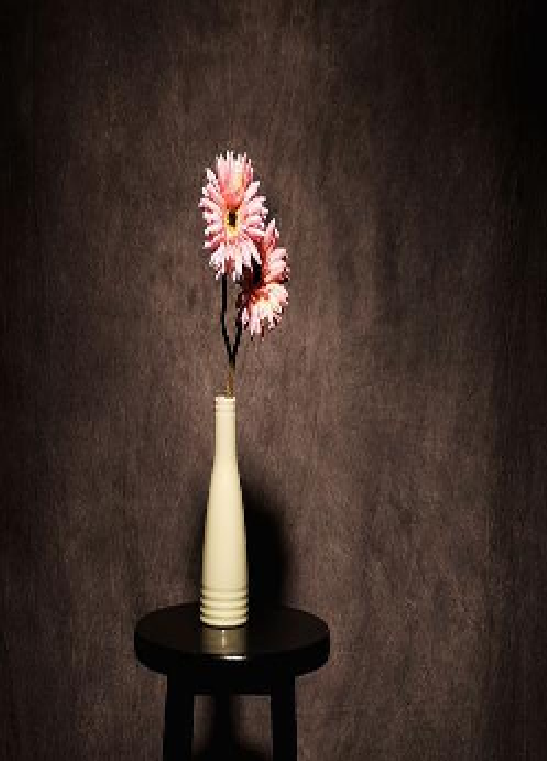
\includegraphics[scale=0.15]{pics/2-2.png}
    \caption{picture1 after scaling}
    \label{pic2-2}
    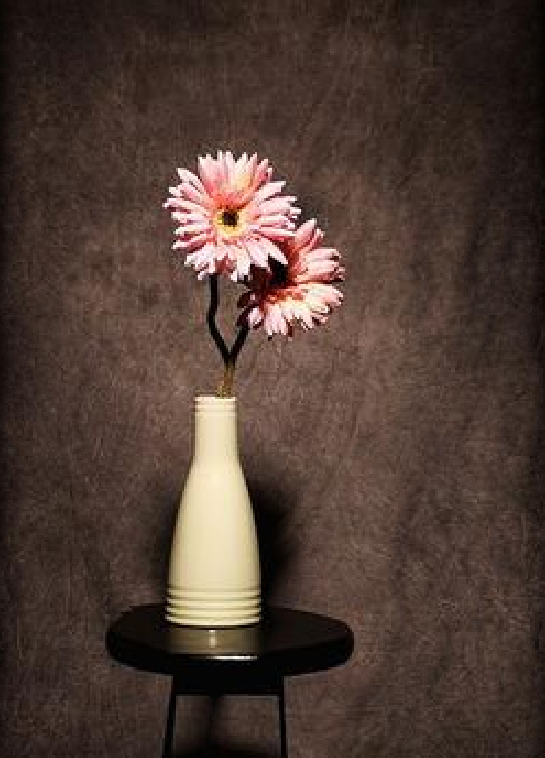
\includegraphics[scale=0.15]{pics/2-3.png}
    \caption{picture1 after Seam Carving}
    \label{pic2-3} 
\end{center}
\end{figure}

Let us check the picture1 \ref{pic2-1} first. This picture has a vase of flowers in the middle. After scaling, we got \ref{pic2-2}. As you can see, the vase and flowers are flattened. Their shapes are transformed into a strange style which is impossible to be seen in reality. That means scaling broke the contents the picture holds at first. However, in \ref{pic2-3}, after being processed by Seam Carving, the vase and flowers are hardly changed, while the width of the picture is reduced to a half of its used to be. This is a successful case of Seam Carving. Nevertheless, corp can realize the same effect as we can imagine. To show the superiority of Seam Carving, let us check the next picture, that's picture2.

\begin{figure}
\begin{center}
   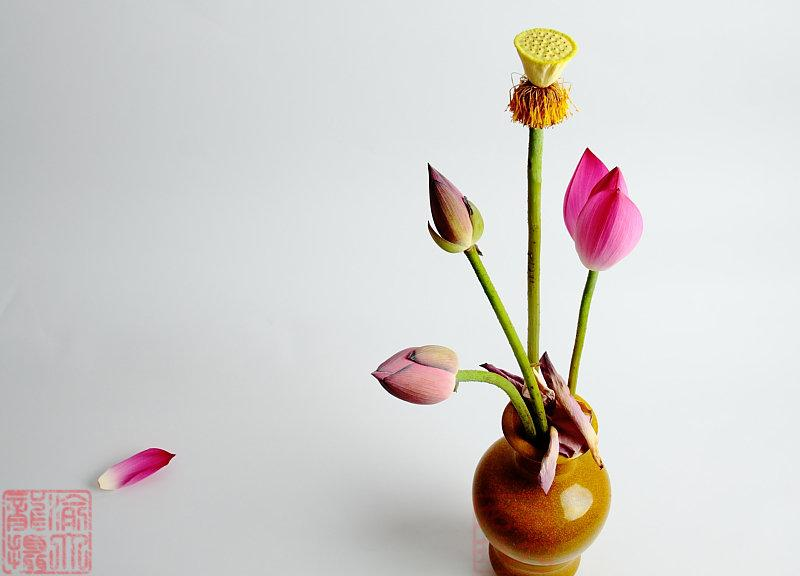
\includegraphics[scale=0.9]{pics/1-1.jpg}
    \caption{The raw picture2}
    \label{pic1-1}
    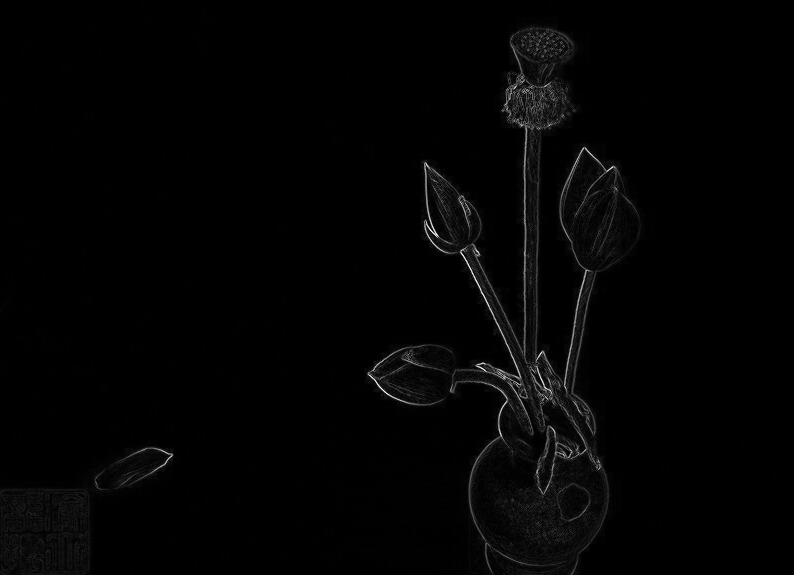
\includegraphics[scale=0.2]{pics/1-0.png}
    \caption{picture2's energy map}
    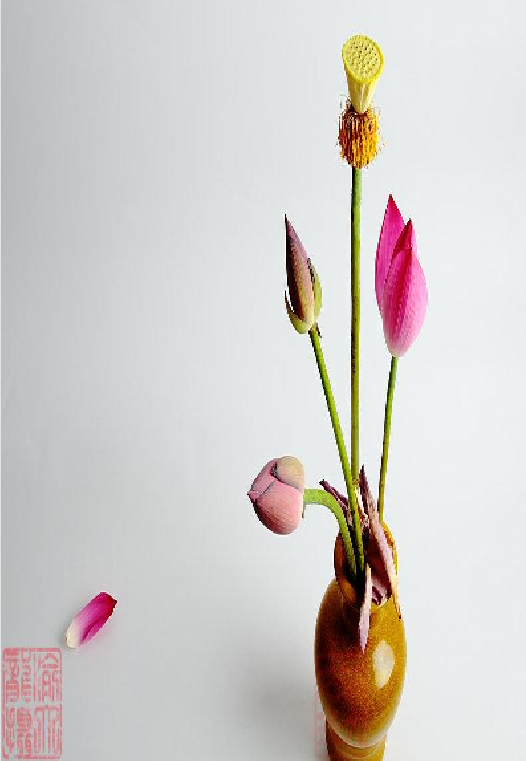
\includegraphics[scale=0.15]{pics/1-2.png}
    \caption{picture2 after scaling}
    \label{pic1-2}
    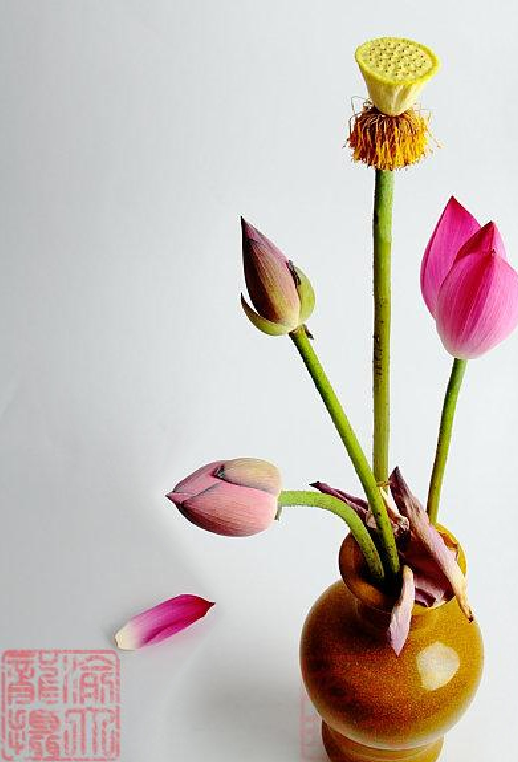
\includegraphics[scale=0.15]{pics/1-3.png}
    \caption{picture2 after Seam Carving}
    \label{pic1-3} 
\end{center}
\end{figure}

As you can see, there are two main objects in picture2 \ref{pic1-1}. One is a vase of flowers in the right side, and the other is a petal and a stamp in the left down side. Scaling \ref{pic1-2} has bad performance, as it changed the shapes of objects in picture. Moreover, we cannot deal the picture with crop. There is few room in the rim of the picture, which means we can hardly crop anything from the picture. If we need to keep the shapes of those objects while reducing its width, we can only crop the middle of the picture, and that will make the picture separate. But when we look at Figure \ref{pic1-3}, the result of Seam Carving, all the requirements are met. 

I hope these cases can help you understand how fancy Seam Carving is.

%--------
\section{Improvement of Seam Carving}
From the above, we have got to know the basic operation of Seam Carving. However, Seam carving also has its disadvantages. Let us take the following picture as an example.

\begin{figure}
\begin{center}
   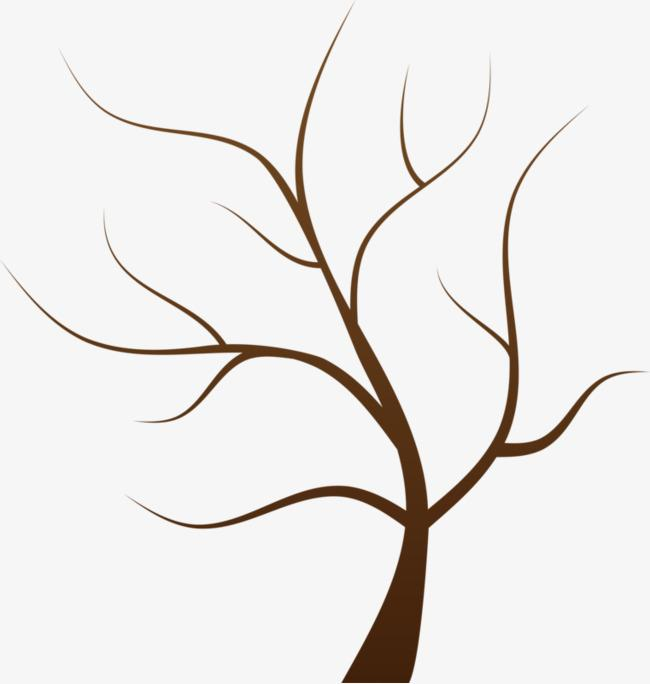
\includegraphics[scale=0.2]{pics/3-1.jpg}
    \caption{The raw picture3}
    \label{pic3-1}
    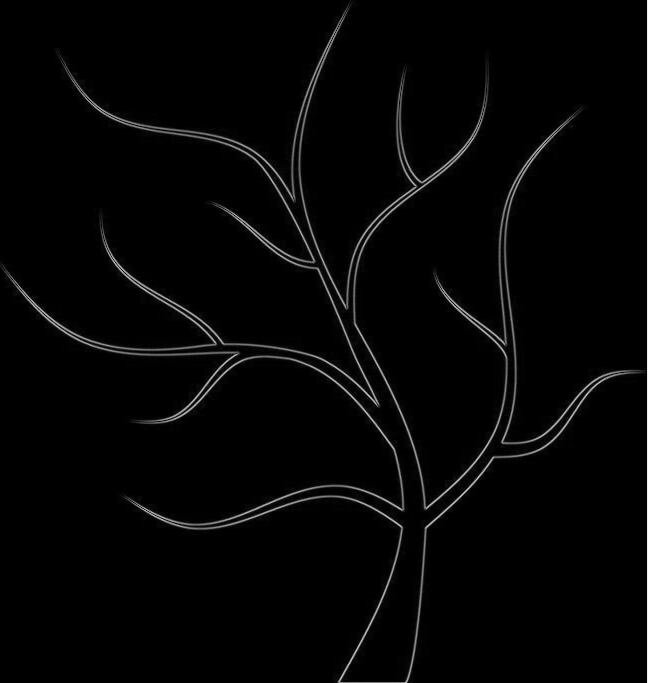
\includegraphics[scale=0.2]{pics/3-0.png}
    \caption{Picture3's energy map}
    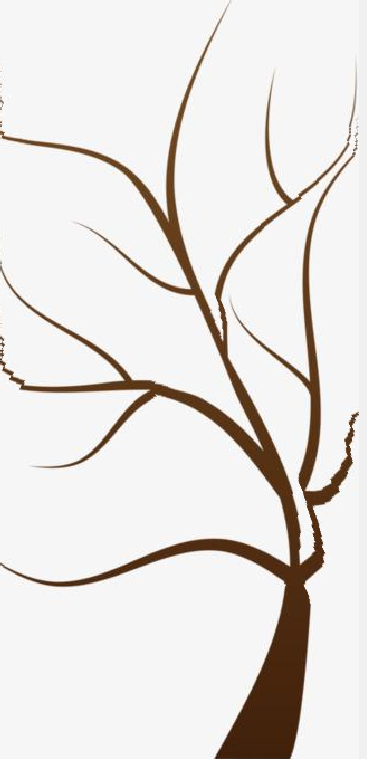
\includegraphics[scale=0.15]{pics/3-2.png}
    \caption{Picture3 after Seam Carving}
    \label{pic3-2}
    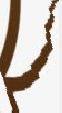
\includegraphics[scale=0.5]{pics/3-3.png}
    \caption{The local amplification}
    \label{pic3-3} 
\end{center}
\end{figure}

There is a bare tree in picture3 \ref{pic3-1}, and the result after Seam Carving has been show in Figure \ref{pic3-2}. If we take a good look at the result, we will find that the result is not that satisfying. Figure \ref{pic3-3} is the local amplification of the result. As you can see in Figure \ref{pic3-3}, some smooth curve got jags after Seam Carving, which will not happen in our reality. That's because for some thin curves, some pixels in the middle of the curve get removed, and that will produce some intervals in the curve. We need to improve Seam Carving algorithm to avoid this.

Take a look at previous Seam Carving algorithm, we can find that the seam we removed is the one that holds least energy. Now consider removing the seam that inserts the least energy to the image, instead of removing the seam of least energy. If we remove one pixel, the two pixels in its right side and left side have similar energy, which means these two pixels are similar, then the new picture will look the same.

To achieve this, we just need to change the calculation method of the matrix $EC$. For a pixel positioned $(i,j)$, $EC(i,j)$ should not only count the value in last pixel $(i',j')$'s cumulate energy $EC(i',j')$, but also the difference value of its both sides, namely $|E(i,j+1)-E(i,j-1)|$. What's more, the vertical difference should also be counted. If the seam goes to right, then add $|E(i-1,j)-E(i,j-1)|$; If it goes to left, then add $|E(i-1,j)-E(i,j+1)|$. The dynamic programming transfer equation is changed into:

$$
E(i,j)=\min
\left\{
\begin{matrix}{}
EC(i-1,j-1)+|E(i,j+1)-E(i,j-1)|\\
+|E(i-1,j)-E(i,j-1)|\\
EC(i-1,j)+|E(i,j+1)-E(i,j-1)|\\
EC(i-1,j+1)+|E(i,j+1)-E(i,j-1)|\\
+|E(i-1,j)-E(i,j+1)|
\end{matrix}
\right.
$$

Respectively correspond to three cases above, the updating method of $PM$ is:

$$
PM_{i,j}=
\left\{\begin{matrix}{}
j-1,\quad case1\\
j,\quad case2\\
j+1,\quad case3\\
\end{matrix}\right.
$$

So here is the new algorithm to calculate $EC$ and $PM$:

\begin{algorithm}[htb]  
  \caption{Calculate $EC$ and $PM$}  
  \begin{algorithmic}[1]  
    \Require
    The energy map $E$;
    The size of raw picture $m\times n$;
    \Ensure  
    The cumulated energy map $EC$; 
    The path map $PM$;
    \State assign$i=1,j=1$;  
    \State assign $tmp1 = EC(i-1,j-1)+|E(i,j+1)-E(i,j-1)|+|E(i-1,j)-E(i,j-1)|$, $tmp2 = EC(i-1,j)+|E(i,j+1)-E(i,j-1)|$, and $tmp3 = EC(i-1,j+1)+|E(i,j+1)-E(i,j-1)|+|E(i-1,j)-E(i,j+1)|$
    \State $EC_{i,j}=\min(tmp1, tmp2, tmp3)$ 
    \State if $EC(i-1,j-1)=tmp1$,$PM_{i,j}=j-1$;if $EC(i-1,j)=tmp2$,$PM_{i,j}=j$;if $EC(i-1,j+1)=tmp3$,$PM_{i,j}=j+1$ 
    \State if $i==m,j==n$, goto return; if $j==n$, then assign $i=i+1,j=1$, goto2; else assign $j=j+1$, goto2.\\
    \Return $EC$, $PM$;
  \end{algorithmic}  
\end{algorithm}

Now change the code like this to achieve the improved Seam Carving method:
\begin{lstlisting}
for j = 2: wid_now-1
    tmp1 = EC(i-1, j-1) + ...
    abs(E(i-1,j+1)-E(i,j-1)) ...
    + abs(E(i-1,j)-E(i,j-1));
    tmp2 = EC(i-1, j) + ...
    abs(E(i,j+1)-E(i,j-1));
    tmp3 = EC(i-1, j+1) + ...
    abs(E(i,j+1)-E(i,j-1)) + ...
    abs(E(i-1,j)-E(i,j+1));
    if tmp1<tmp2 && tmp1<tmp3
        EC(i, j) = tmp1;
        PM(i, j) = j-1;
    elseif tmp2<tmp1 && tmp2<tmp3
        EC(i, j) = tmp2;
        PM(i, j) = j;
    else
        EC(i, j) = tmp3;
        PM(i, j) = j+1;
    end
end
\end{lstlisting}

Processing the same picture by the improved method, we can get the Figure \ref{pic3-4}. Compared to Figure \ref{pic3-2} we can easily find, the result of the improved version has smoother curve, and less jags. Obviously it is more natural and in line with people's intuitive feelings. The improved version has better performance than the previous version.

%---------

\section{Conclusion}
Seam Carving is a content-aware algorithm for picture resizing. Compared to traditional approaches of picture resizing such as crop and scale, Seam Carving can keep the shapes of important objects in the picture as much as possible, so that after resizing, these objects are still conform to reality. By calculate the energy map of the input picture, which is defined by gradient, we can remove a seam from the picture which has least energy. That means each time, we just delete a path in the picture which contain the least information. By doing this over and over again, we can resize the picture while keep the important parts as the same as they used to be.

\begin{figure}
\begin{center}
    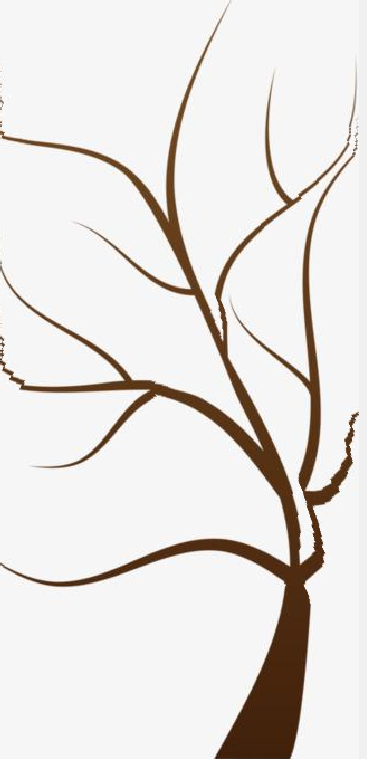
\includegraphics[scale=0.2]{pics/3-2.png}
    \caption{Picture3 after Seam Carving}
    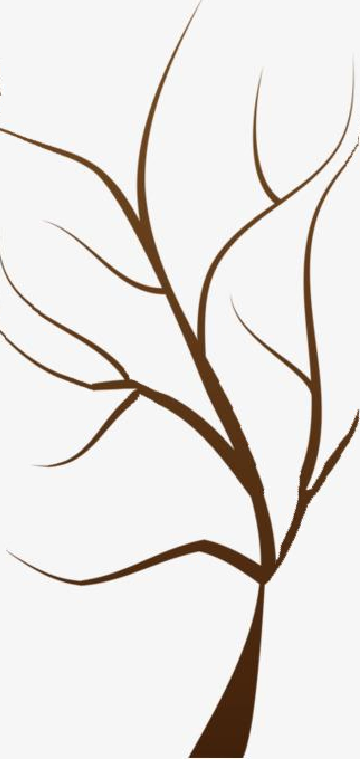
\includegraphics[scale=0.2]{pics/3-4.png}
    \caption{Picture3 after improved Seam Carving}
    \label{pic3-4} 
\end{center}
\end{figure}


\begin{thebibliography}{99}  

\bibitem{ref4}Seam carving for content-aware image resizing[J]. Tog, 2007.

\bibitem{ref1}LIANG Xiao-li, SUN Hong-Lin. Image zooming based on linear interpolation and its realization[J]. Journal of Changsha Telecommunications and Technology Vocational College, 2008, 7(2):49-49.
\bibitem{ref2}LI Yan-Lin. Nearest Neighbor Scaling Principle and Realization of Image[J]. Journal of Changzhi University, 2016, 33(005):31-32.
\bibitem{ref3}MA Tian-jun, GAO You-xing. Image Enlargment via Spline-Based Nonuniform Interpolation[J]. Electronic Science, 2004(02):45-47.

\end{thebibliography} 

\end{document}
